\section{WIMPs pair production}
    \label{sec:WIMPsProduction}

In this section, the results of the monojet analysis are converted into limits on the pair production of WIMPs. 
Samples for several models based on an effective theory (D5, D8 and D9, see Table~\ref{tab:WIMPsEffectiveOperators}) corresponding to the process $\wimpwimp$ have been generated.
They are implemented using LO matrix elements in \madgraph{}.
The WIMP pair production plus one or two additional partons from ISR/FSR is considered.
For each operator, a sample is generated requiring at least one parton with $\pt>\unit[80]{GeV}$, and another sample is generated with at least one parton with a minimum $\pt$ of 300~GeV.
The latter samples are needed to populate those signal regions with $\met$ requirements larger than 350~GeV.
Only initial states of the four lightest quarks are considered, assuming equal coupling strengths for all quark flavors to the WIMPs.
The generated events are interfaced to \pythia{} for the parton showering and hadronization.
The MLM prescription is used for matching the matrix element calculations to the parton shower evolution.
The PDF set CTEQ6L1 is used for the event simulation, and the renormalization and factorization scales are set to the geometric average of $m_{\chi}^2 + \pt^2$ for the two WIMPs, being $m_{\chi}$ is the mass of the WIMP.
Events with WIMP masses between $\unit[10]{GeV}$ and $\unit[1.3]{TeV}$ are simulated for the different effective operators considered.

To study the transition between the effective field theory and a physical renormalizable model for Dirac fermion WIMPs coupling to SM particles via a new mediator particle $Z'$, a simplified model is generated with \madgraph{}.
For each WIMP mass, mediator particle masses $M_{\text{med}}$ between $\unit[50]{GeV}$ and $\unit[13]{TeV}$ are considered, for two different mediator particle width each ($\Gamma_{\text{med}} = M_{\text{med}}/3$ and $\Gamma_{\text{med}} = M_{\text{med}}/8\pi$).
  
For each effective model, the limits are extracted from the signal region M3, since it has the best expected sensitivity.
This is translated into corresponding 90\% CL limits\footnote{The limits are extracted at 90\% CL instead of 95\% CL, in order for them to be compared to direct dark matter search experiments.} on the suppression scale $M^{\ast}$ as a function of $m_{\chi}$.
To derive the lower limits in $M^{\ast}$, the $CL_s$ approach described in Section~\ref{sec:ComputationOfLimits} is used.
    
The systematic uncertainties for these models are computed as described in Chapter~\ref{chapter:Interpretations}.
Experimental uncertainties on jets and $\met$ scale and resolution, lepton efficiency, and luminosity translate into a 5\% to 3\% uncertainty on the signal yields for D5 and D8 models for a WIMP masses between 50~GeV and 1.3~TeV.
For the model D9, the experimental uncertainty varies from 1.5\% to 4\% for the same WIMP mass range.
The theoretical uncertainties include: the uncertainty on the renormalization, factorization scales; the uncertainty on the matrix element to parton shower matching scales; the uncertainty on the modeling of the ISF/FSR and the uncertainty on the PDFs.
These uncertainties translate to an effect between 3\% to 8\% in the signal yield, depending on the operator and the WIMP mass.
    
The 90\% CL limits on $M^{\ast}$ for the operators D5 (vector), D8 (axial-vector) and D9 (tensor) are reported in Table~\ref{tab:WIMPsEffective_limit_mstar} and shown in Figure~\ref{fig:WIMPsEffectiveMstar}, down to WIMP masses of 10~GeV.
These limits are extrapolated even further to smaller $m_{\chi}$ values, since for such low-mass WIMPs there is a negligible change in the fiducial cross section and kinematic distributions.

%--- \ref{tab:WIMPsEffective_limit_mstar}
\begin{sidewaystable}[h!]
\centering
\begin{tabular}{c|cc|cc|cc}
\hline\hline
\multirow{2}{*}{{\bf $\mathbf{m_\chi}$ [GeV]}} & \multicolumn{2}{c|}{\bf $\mathbf{M^*}$ D5 (vector)} & \multicolumn{2}{c|}{\bf $\mathbf{M^*}$ D8 (axial-vector)} & \multicolumn{2}{c}{\bf $\mathbf{M^*}$ D9 (tensor)}\\ 
\cline{2-7}
           & {\bf Obs. [GeV]} & {\bf Exp. [GeV]} & {\bf Obs. [GeV]} & {\bf Exp. [GeV]} & {\bf Obs. [GeV]} & {\bf Exp. [GeV]}\\ 
\hline
    1      &    990 &   992 &   971 &   973 &   1672    &   1677    \\
    10     &    990 &   992 &   971 &   973 &   1672    &   1677    \\
    50     &    990 &   992 &   971 &   973 &   1715    &   1719    \\
    100 &   979 &   982 &   948 &   950 &   1613    &   1618    \\
    200 &   957 &   960 &   893 &   893 &   1541    &   1545    \\
    400 &   896 &   899 &   760 &   763 &   1294    &   1297    \\
    700 &   706 &   708 &   544 &   545 &   922 &   923 \\
    1000    &   507 &   509 &   367 &   369 &   634 &   636 \\
    1300    &   344 &   345 &   229     &   230     &   430 &   431     \\
    \hline\hline
    \end{tabular}
    \caption[The 90\% CL observed and expected limits on $M^*$ as a function of the WIMP mass $m_\chi$ for different interaction models.]{The 90\% CL observed and expected limits on $M^*$ as a function of the WIMP mass $m_\chi$ for D5 (vector), D8 (axial-vector) and D9 (tensor) interaction models.}
    \label{tab:WIMPsEffective_limit_mstar}
    \end{sidewaystable}



The effective theories used are based on the assumption that a new mediator particle couples SM particles to pairs of WIMPs, and that the mass of the mediator is much larger than the scale of the interaction.
If this is the case, the mediator cannot be produced directly in the collisions, and therefore it can be integrated out by the effective formalism.
However, this assumption is not always correct at the LHC, where the momentum transfer can reach the TeV energies.
For a given operator, one possible validity criterion would be that the momentum transferred in the hard interaction, $Q_{\text{tr}}$ is below the mediator mass, $M_{\text{med}}$, defined as $M_{\text{med}} = \sqrt{g_{q} g_{\chi}} M^{\ast}$, where $g_{q}$ and $g_{\chi}$ are the couplings of the mediator to the SM particles and the WIMPs, respectively.
Figure~\ref{fig:WIMPsEffectiveMstar} also shows the 90\% CL upper limit on $M^{\ast}$ when this ``truncation'' criteria ($Q<M_{\text{med}}$) is imposed, assuming $\sqrt{g_{q} g_{\chi}} = 1$.
The truncated limits fulfill the respective validity criteria wherever the lines are drawn in the figure.
For D5 (D9) for example, the criterion is fulfilled for WIMP masses up to 100~GeV (200~GeV).
No attempt is made to consider different couplings than $\sqrt{g_{q} g_{\chi}} = 1$ in these effective models.
The limits on $M^{\ast}$ for the truncated effective models are also quoted in Table~\ref{tab:WIMPsEffective_limit_mstar_trunc}.
The thermal relic lines are also included from Ref.~\cite{Goodman:2010ku} to this figure, corresponding to a coupling, set by $M^{\ast}$, of WIMPs to quarks such that WIMPs have the correct relic abundance as measured by the WMAP satelite~\cite{Larson:2010gs}, in the absense of any other interaction, apart from the one considered.

%--- \ref{tab:WIMPsEffective_limit_mstar_trunc}
\begin{table}[ht!]
   \centering
\begin{tabular}{ccc}
\hline\hline
{\bf $\mathbf{m_{\chi}}$ [GeV]} & {\bf $\mathbf{M^*}$ [GeV] D5 (vector)} & {\bf $\mathbf{M^*}$ [GeV] D9 (tensor)} \\ 
\hline
1	   &	600	&		-	      \\
10	   &	650	&		1600   	\\
25	   &	650	&		-         \\
50	   &	600	&		1650   	\\
100	   &	550	&		1550   	\\
200	   &	-   &		1450   	\\
\hline\hline
\end{tabular}
\caption{90\% CL Observed limit on $M^*$ for D5 and D9 models, with truncation of the events with $\sqrt{\hat{s}}>M^*$.}
\label{tab:WIMPsEffective_limit_mstar_trunc}
\end{table}


\begin{figure}[!t] 
   \centering
   \mbox{
   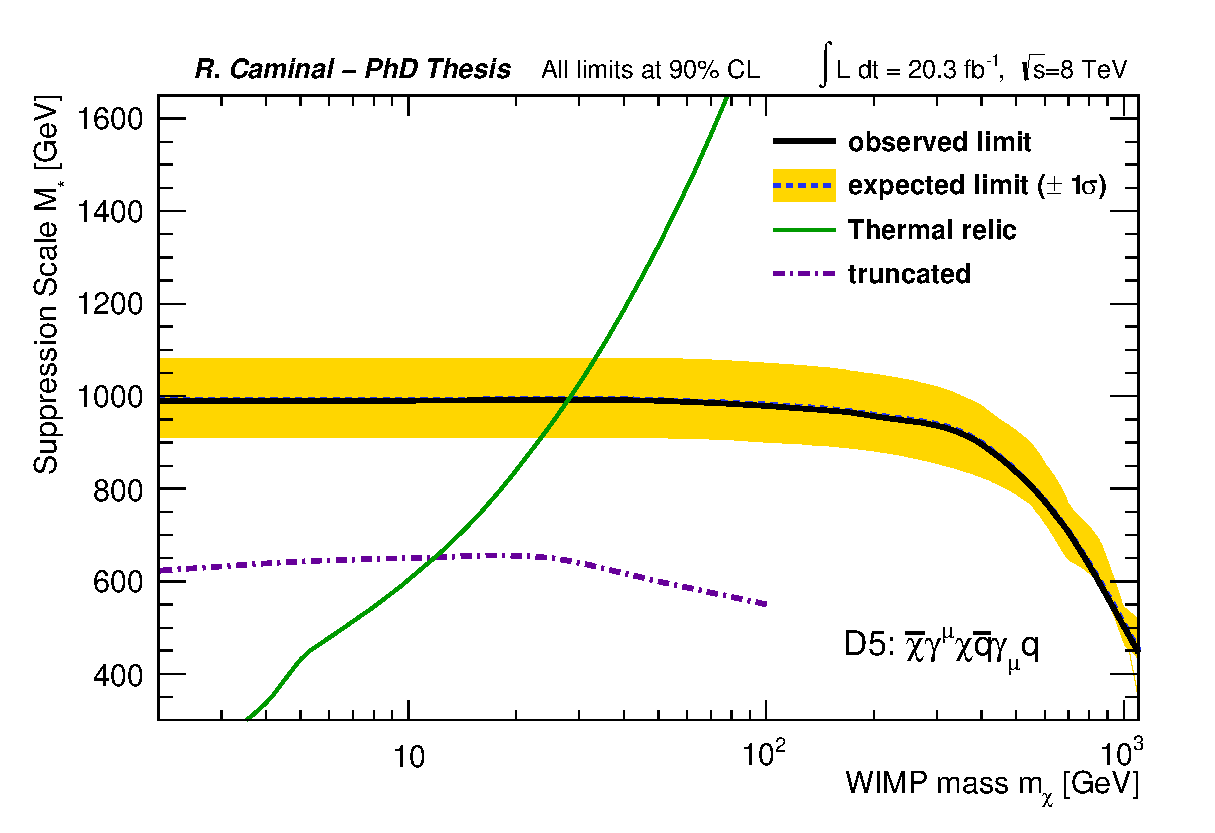
\includegraphics[width=0.495\textwidth]{Interpretations/Figures/WIMPmStar_D5.eps} 
   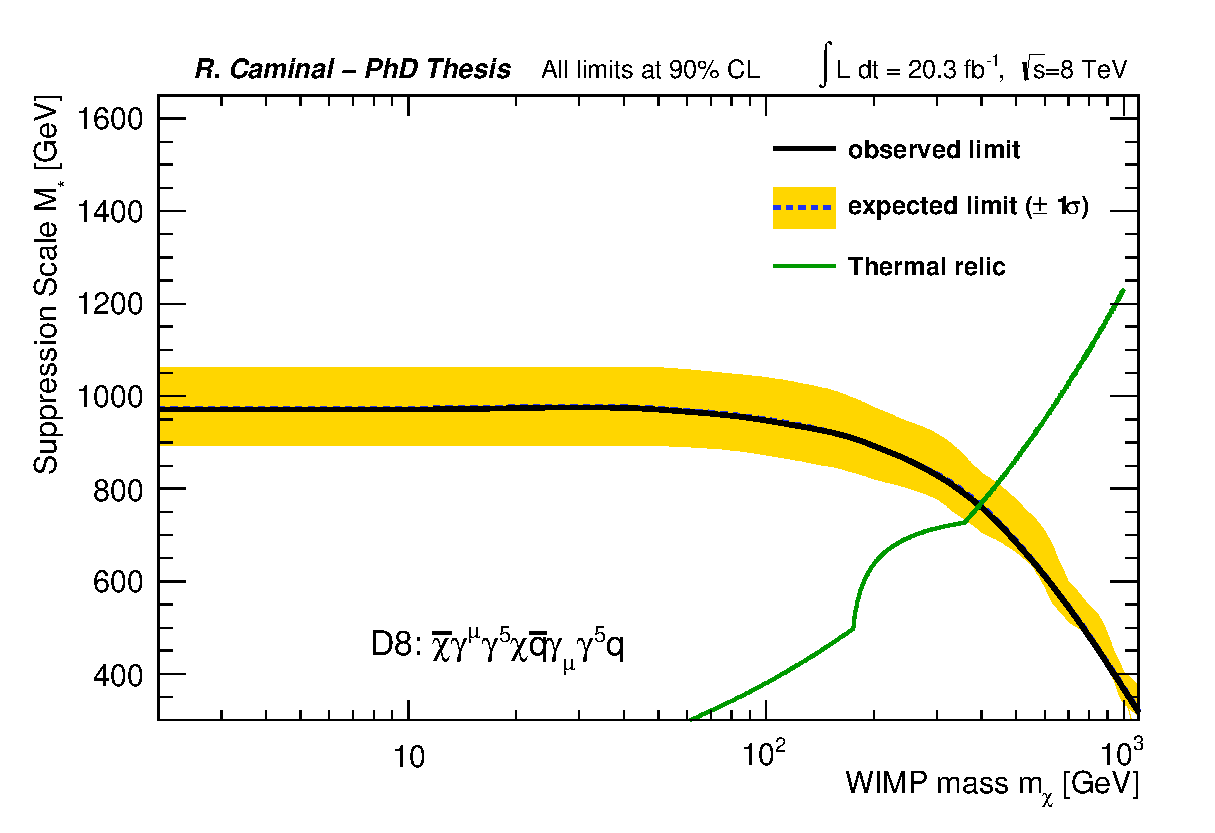
\includegraphics[width=0.495\textwidth]{Interpretations/Figures/WIMPmStar_D8.eps} 
   }
   \mbox{
   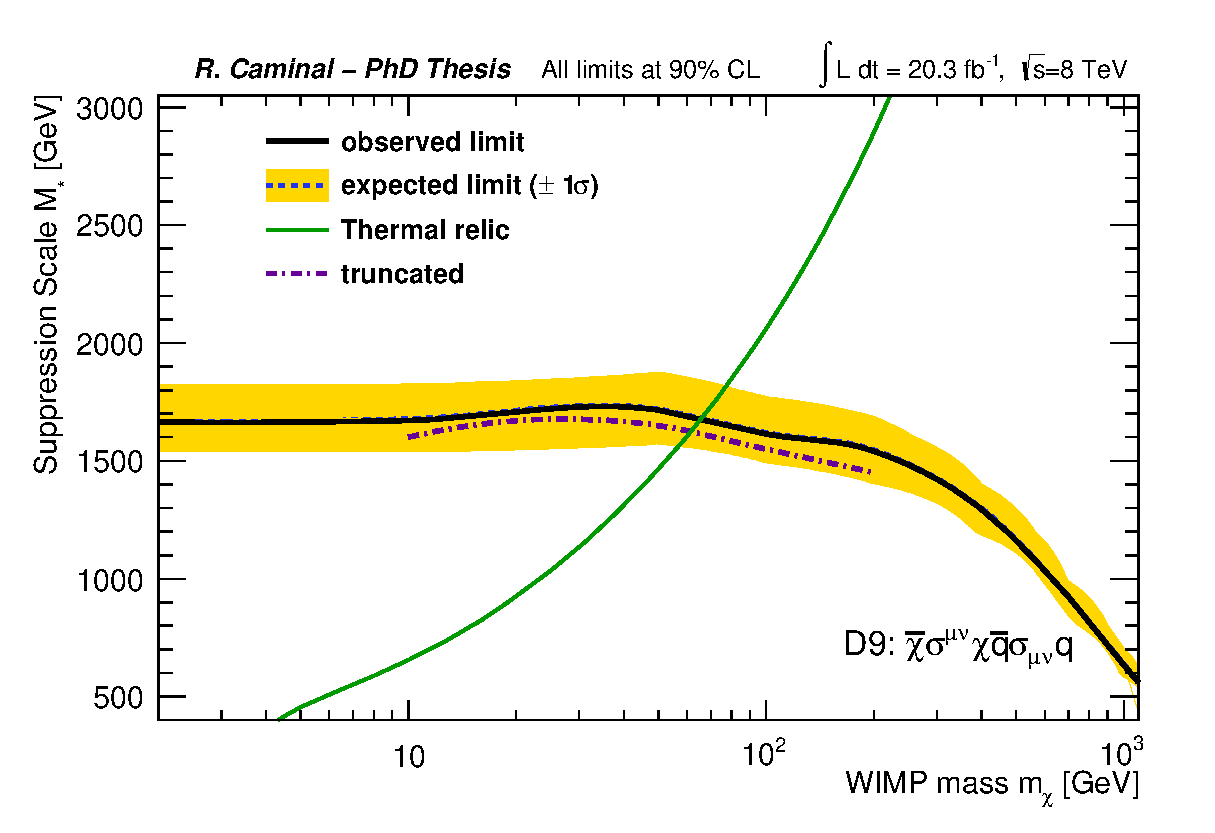
\includegraphics[width=0.495\textwidth]{Interpretations/Figures/WIMPmStar_D9.eps} 
   }
   \caption[Observed and expected 90\% CL limits on $M^*$ as a function of the WIMP mass $m_\chi$ for different operators in the selection M3.]{Expected and observed 90\% CL limits on $M^{\ast}$ as a function of the WIMP mass $m_\chi$ for an integrated luminosity of 20.3~\ifb for the D5 (vector), D8 (axial-vector) and D9 (tensor) operators in the M3 signal region. The Expected and observed limits are shown as dashed blue and solid black lines, respectively.
     The $\pm 1\sigma$ error band in yellow around the expected limit is due to the acceptance uncertainties (both experimental and theoretical). The rising green lines are the $M^{\ast}$ values at which WIMPs of the given mass result in the relic density as measured by WMAP~\cite{Larson:2010gs}, assuming annihilation in the early universe proceeded exclusively via the given operator.
     The thermal relic line for D8 has a bump feature at the top quark mass where the annihilation channel to top quarks opens.
     The purple dot-dashed  line is the 95\% CL observed limit on $M^{\ast}$ imposing a validity criterion with a coupling strength of 1.}
   \label{fig:WIMPsEffectiveMstar}
\end{figure}

A way to avoid the validity issues of the effective theories is to use a simplified model which includes a mediator explicitly.
Here as an example, a vector-like $Z'$ boson is considered, corresponding to the D5 operator in the effective theory framework, of a given mass, $M_{\text{med}}$, and width, $\Gamma_{\text{med}}$.
With this approach, the product of the coupling constants of the $Z'$ can be constrained.
Figure~\ref{fig:WIMPsSimplifiedCouplingLimit} shows the 90\% CL limits on $\sqrt{g_{q}g_{\chi}}$ as a function of $M_{\text{med}}$ for different values of the WIMP mass and the width of the mediator.
Couplings above 1 and 1.5 are excluded for WIMP masses between 25~GeV and 400~GeV, respectively, for mediator masses between 25~GeV and around 1~TeV.
For higher mediator masses, the limits on the couplings have higher values.
In particular, for mediator masses around 10~TeV, the couplings enter the non-perturbative regime and the theory is not anymore valid, for any WIMP mass and mediator width configuration.

\begin{figure}[!t]
  \begin{center}
    \mbox{
      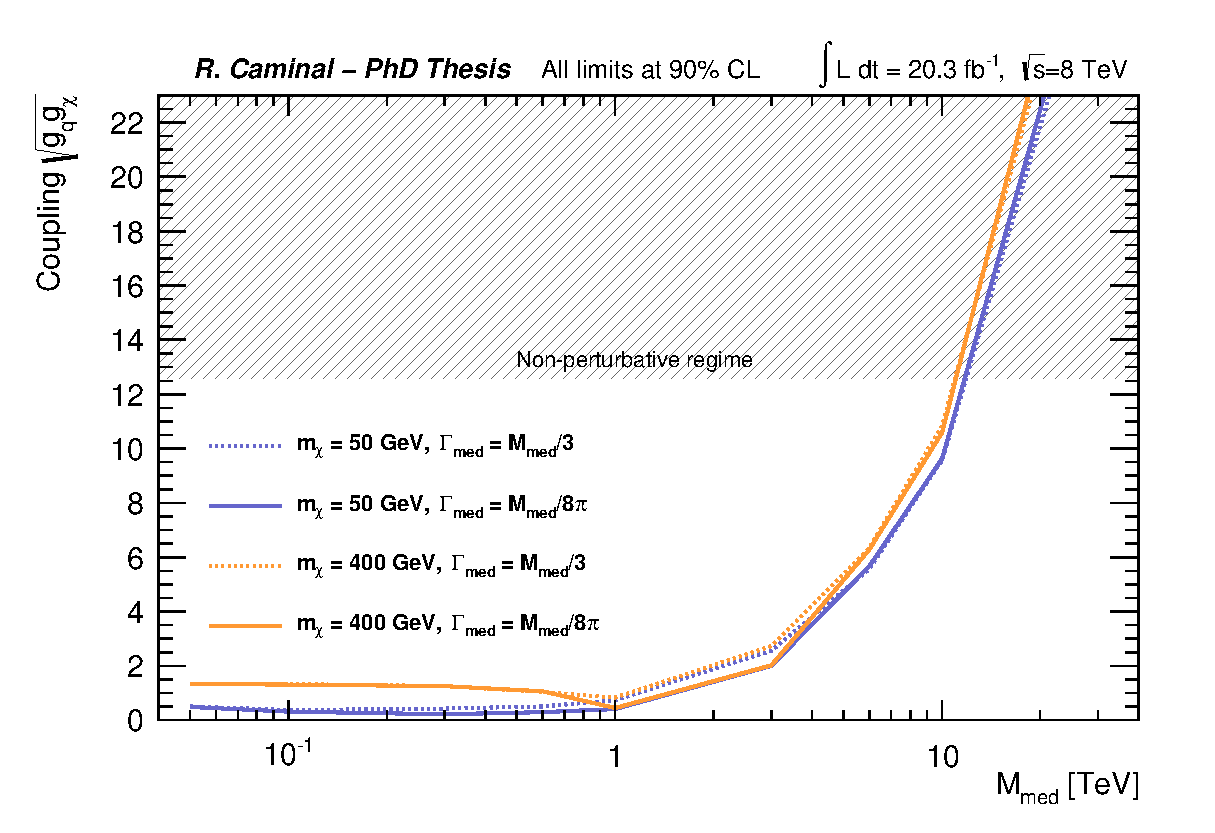
\includegraphics[width=0.795\textwidth]{Interpretations/Figures/WIMPsimplified_MmedCoupling.eps}
    }
  \end{center}
  \caption[Observed 90\% CL limits on the product of the coupling constants as a function of the mediator mass, assuming a $Z'$-like simplified model.]{Observed 90\% CL limits on the product of the coupling constants, $\sqrt{g_q g_\chi}$, as a function of the mediator mass, $M_\text{med}$, assuming a $Z'$-like simplified model and a DM mass of 50~GeV and 400~GeV. The width of the mediator is varied between $M_\text{med}/3$ and $M_\text{med}/8\pi$.}
  \label{fig:WIMPsSimplifiedCouplingLimit}
\end{figure}

These limits can be translated into 90\% CL limits on $M^{\ast}$ as a function of $M_{\text{med}}$.
Figure~\ref{fig:WIMPsSimplifiedMstarLimit} demonstrates how for a given mediator particle mass and two values of the width, the real value of the mass suppression scale would compare to the $M^{\ast}$ derived assuming a contact interaction (shown as dashed line in the figure).
This contact interaction regime is reached by values of the $M_{\text{med}}$ larger than 5~TeV.
In the $\unit[700]{GeV} < M_\text{med} < \unit[5]{TeV}$ the mediator would be produced resonantly, and therefore the actual $M^{\ast}$ value is higher than in the contact interaction regime.
For lower mediator masses, the limit on $M^{\ast}$ is very low, since the WIMP would be heavier than the mediator, and the WIMP pair production via this mediator would be kinematically suppressed.
In this region, the contact interaction limits would be optimistic and overestimate the actual $M^{\ast}$ values.

\begin{figure}[!t]
  \begin{center}
    \mbox{
      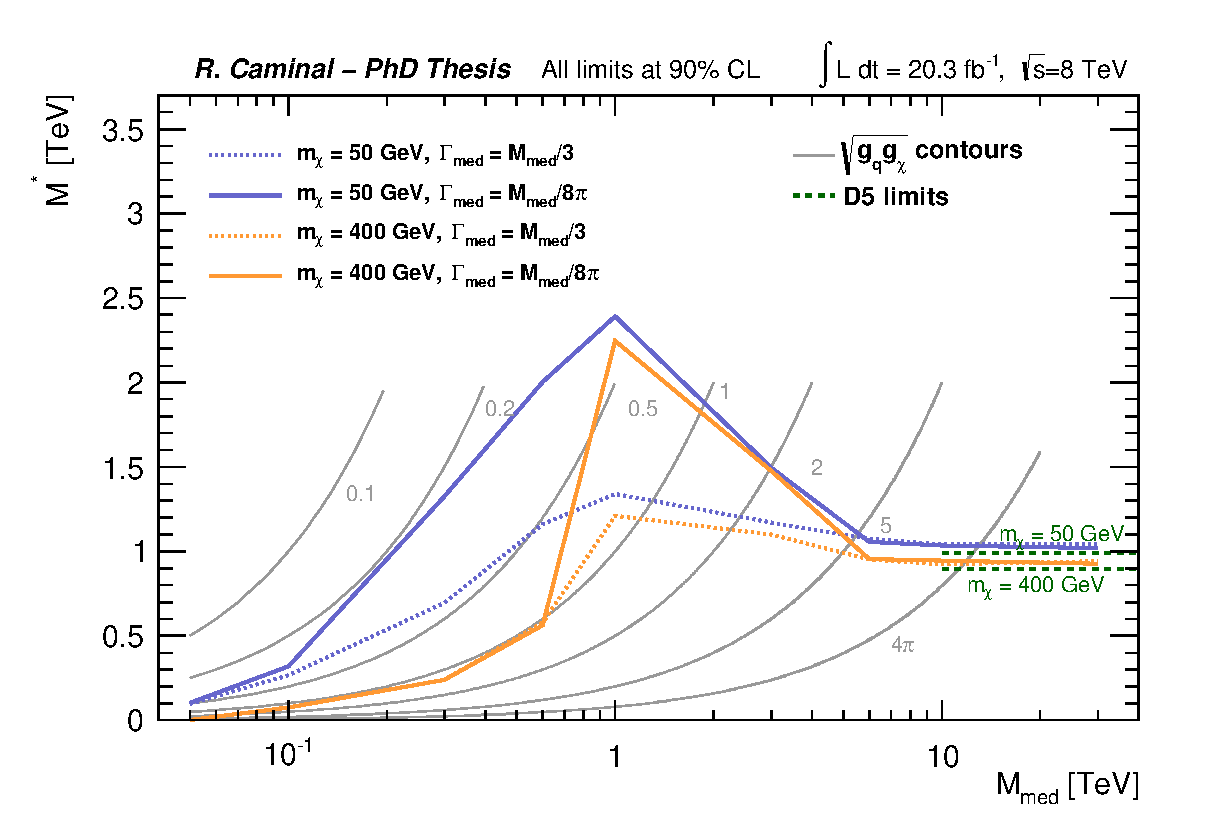
\includegraphics[width=0.795\textwidth]{Interpretations/Figures/WIMPsimplified_MstarMmed_vector.eps}
    }
  \end{center}
  \caption[Observed limits on $M^{\ast}$ as a function of the mediator mass assuming a $Z'$-like simplified model.]{Observed limits on $M^{\ast}$ as a function of the mediator mass, $M_\text{med}$, assuming a $Z'$-like simplified model and a DM mass of 50~GeV and 400~GeV.
  The width of the mediator is varied between $M_\text{med}/3$ and $M_\text{med}/8\pi$.
  The corresponding limits of the effective model D5 are shown as dashed lines.
  Contour lines indicating a range of values of the product of the coupling constants, $\sqrt{g_q g_\chi}$, are also shown.}
  \label{fig:WIMPsSimplifiedMstarLimit}
\end{figure}

In the effective operator approach, the bounds on $M^{\ast}$ for a given $m_{\chi}$ can be converted to bounds on WIMP-nucleon scattering cross section, $\sigma_{\chi N}$, probed by direct DM experiments, using the transformation equations \ref{eq:WIMP-Nucleon}:

\begin{equation}
\begin{split}
\sigma^{D5}_{\chi N} &= 1.38 \times \unit[10^{-37}]{cm^2} \times \left(\frac{\mu_{\chi}}{\unit[1]{GeV}}\right)^2\left(\frac{\unit[300]{GeV}}{M^{\ast}}\right)^4 \\
\sigma^{D8}_{\chi N} &= 4.70 \times \unit[10^{-40}]{cm^2} \times \left(\frac{\mu_{\chi}}{\unit[1]{GeV}}\right)^2\left(\frac{\unit[300]{GeV}}{M^{\ast}}\right)^4 \\
\sigma^{D9}_{\chi N} &= 4.70 \times \unit[10^{-40}]{cm^2} \times \left(\frac{\mu_{\chi}}{\unit[1]{GeV}}\right)^2\left(\frac{\unit[300]{GeV}}{M^{\ast}}\right)^4. \\
\end{split}
\label{eq:WIMP-Nucleon_2}
\end{equation}

These bounds describe the scattering of WIMPs from nucleons at a very low momentum transfer, of the order of the keV.
Depending on the type of interaction, contributions to spin-dependent and spin-independent WIMP-nucleon interactions are expected.
The 90\% CL lower limits on the WIMP-nucleon scattering cross section are shown in Figure~\ref{fig:WIMPsNucleonXSection}.
Under the assumption made by the effective approach, these limits are relevant in the low DM mass region, and remain important in the full $m_{\chi}$ range covered.
Cross sections above $\unit[2.7\times10^{-40}]{cm^{2}}$ ($\unit[7.0\times10^{-38}]{cm^{2}}$) are excluded for WIMP masses of 1~GeV (1.3~TeV), respectively.
The spin-dependent limits in this figure are based on D8 and D9, where for D8 the limits have been calculated with the D5 acceptances, since they are identical, together with the D8 production cross section.
Both limits are significantly stronger than those from direct-detection experiments.
For D8, cross sections above $\unit[1.0\times10^{-41}]{cm^{2}}$ ($\unit[1.2\times10^{-38}]{cm^{2}}$) are excluded at 90\% CL for WIMP masses of 1~GeV (1.3~TeV), respectively, while for D9, cross sections above $\unit[1.1\times10^{-42}]{cm^{2}}$ ($\unit[9.8\times10^{-40}]{cm^{2}}$) are excluded in the same WIMP mass range.
The limits on the non-truncated and truncated $\sigma_{\chi N}$ are also shown in Tables~\ref{tab:WIMPsEffective_limit_sigma} and~\ref{tab:WIMPsEffective_limit_sigma_truncated}, respectively.

%--- \ref{tab:WIMPsEffective_limit_sigma}
\begin{sidewaystable}[h!]
   \centering
\begin{tabular}{c|cc|cc|cc}
\hline\hline
\multirow{2}{*}{{\bf $\mathbf{m_\chi}$ [GeV]}} & \multicolumn{2}{c|}{{\bf $\mathbf{\sigma_{\chi N}}$(D5)}} & \multicolumn{2}{c|}{{\bf $\mathbf{\sigma_{\chi N}}$(D8)}} & \multicolumn{2}{c}{{\bf $\mathbf{\sigma_{\chi N}}$(D9)}}\\ 
\cline{2-7}
       & {\bf Obs. [GeV]} & {\bf Exp. [cm$^2$]} & {\bf Obs. [cm$^2$]} & {\bf Exp. [cm$^2$]} & {\bf Obs. [cm$^2$]} & {\bf Exp. [cm$^2$]}\\ 
\hline
1	   &	2.73$\times 10^{-40}$	&	2.71$\times 10^{-40}$	&	1.00$\times 10^{-41}$	&	9.95$\times 10^{-42}$	&	1.14$\times 10^{-42}$	&	1.13$\times 10^{-42}$	\\
10	   &	8.56$\times 10^{-40}$	&	8.49$\times 10^{-40}$	&	3.15$\times 10^{-41}$	&	3.13$\times 10^{-41}$	&	3.58$\times 10^{-42}$	&	3.54$\times 10^{-42}$	\\
50	   &	9.87$\times 10^{-40}$	&	9.79$\times 10^{-40}$	&	3.63$\times 10^{-41}$	&	3.60$\times 10^{-41}$	&	3.73$\times 10^{-42}$	&	3.70$\times 10^{-42}$	\\
100	&	1.05$\times 10^{-39}$	&	1.04$\times 10^{-39}$	&	4.07$\times 10^{-41}$	&	4.04$\times 10^{-41}$	&	4.86$\times 10^{-42}$	&	4.80$\times 10^{-42}$	\\
200	&	1.16$\times 10^{-39}$	&	1.15$\times 10^{-39}$	&	5.22$\times 10^{-41}$	&	5.17$\times 10^{-41}$	&	5.89$\times 10^{-42}$	&	5.83$\times 10^{-42}$	\\
400	&	1.52$\times 10^{-39}$	&	1.50$\times 10^{-39}$	&	1.00$\times 10^{-40}$	&	9.84$\times 10^{-41}$	&	1.19$\times 10^{-41}$	&	1.18$\times 10^{-41}$	\\
700	&	3.95$\times 10^{-39}$	&	3.91$\times 10^{-39}$	&	3.81$\times 10^{-40}$	&	3.79$\times 10^{-40}$	&	4.63$\times 10^{-41}$	&	4.61$\times 10^{-41}$	\\
1000	&	1.49$\times 10^{-38}$	&	1.46$\times 10^{-38}$	&	1.84$\times 10^{-39}$	&	1.80$\times 10^{-39}$	&	2.07$\times 10^{-40}$	&	2.05$\times 10^{-40}$	\\
1300	&	7.02$\times 10^{-38}$	&	6.94$\times 10^{-38}$	&	1.22$\times 10^{-38}$ 	&	1.20$\times 10^{-38}$ 	&	9.79$\times 10^{-40}$	&	9.70$\times 10^{-40}$ 	\\
\hline\hline
\end{tabular}
\caption[The 90\% CL observed and expected limits on the WIMP-Nucleon scattering cross-section $\sigma_{\chi N}$ as a function of the WIMP mass $m_\chi$ for different interaction models.]{The 90\% CL observed and expected limits on the WIMP-Nucleon scattering cross-section $\sigma_{\chi N}$ as a function of the WIMP mass $m_\chi$ for D5 (vector), D8 (axial-vector) and D9 (tensor) interaction models.}
\label{tab:WIMPsEffective_limit_sigma}
\end{sidewaystable}



%--- \ref{tab:WIMPsEffective_limit_sigma_truncated}
\begin{table}[ht!]
   \centering
\begin{tabular}{ccc}
\hline\hline
$\mathbf{m_{\chi}}$ \textbf{[GeV]}               & {\bf $\mathbf{\sigma_{\chi N}}$(D5)} & {\bf $\mathbf{\sigma_{\chi N}}$(D9)} \\ 
\hline
1	   &	2.02$\times 10^{-39}$	&		-        	            \\
10	   &	4.61$\times 10^{-39}$	&		4.27$\times 10^{-42}$	\\
25	   &	5.12$\times 10^{-39}$	&		-        	            \\
50	   &	7.31$\times 10^{-39}$	&		4.36$\times 10^{-42}$	\\
100	   &	1.06$\times 10^{-38}$	&		5.70$\times 10^{-42}$	\\
200	   &	-                    	&		7.51$\times 10^{-42}$	\\
\hline\hline
\end{tabular}
\caption[The 90\% CL Observed limit on WIMP-nucleon cross section for D5 and D9 models, with truncation of the events with $\sqrt{\hat{s}}>M^*$.]{The 90\% CL Observed limit on WIMP-nucleon cross section, $\sigma_{\chi-N}$, for D5 and D9 models, with truncation of the events with $\sqrt{\hat{s}}>M^*$.}
\label{tab:WIMPsEffective_limit_sigma_truncated}
\end{table}


\begin{figure}[ht] 
   \centering
   \mbox{
     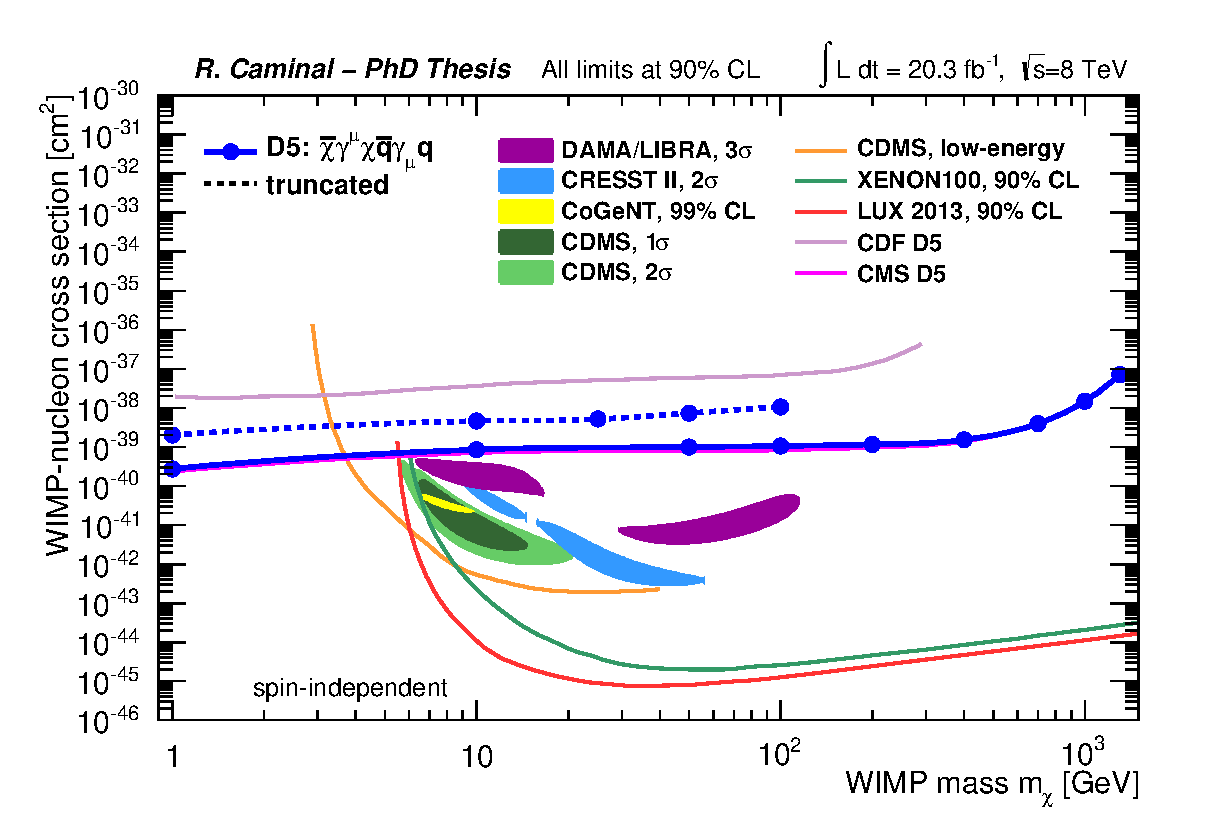
\includegraphics[width=0.795\textwidth]{Interpretations/Figures/WIMPnucleonXsection_spinIndependent.eps} 
   }
   \mbox{
     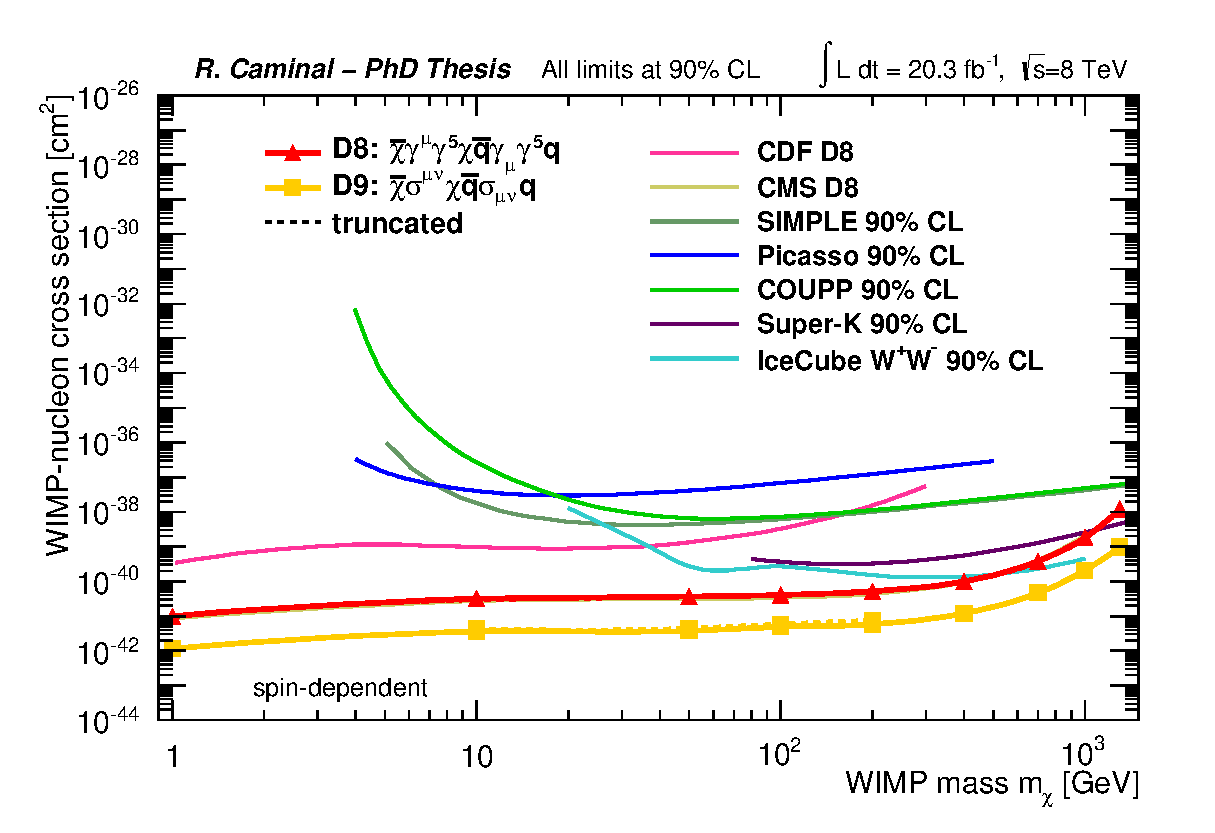
\includegraphics[width=0.795\textwidth]{Interpretations/Figures/WIMPnucleonXsection_spinDependent.eps} 
   }
\caption[90\% CL lower limits on spin-independent and spin-dependent the WIMP-nucleon scattering cross section.]{The 90\% CL lower limits on spin-independent (top) and spin-dependent (bottom) WIMP-nucleon scattering cross section for different masses of $\chi$ in M3 signal region. 
 Results from direct detection experiments for the spin-independent~\cite{Angloher:2011uu,Akerib:2013tjd,Agnese:2013rvf,Agnese:2014aze,Aalseth:2014jpa,Bernabei:2008yi,Bernabei:2010mq,Aprile:2012nq,Aprile:2013doa} and spin-dependent~\cite{Archambault:2012pm,Desai:2004pq,Abbasi:2009uz,Behnke:2010xt,Felizardo:2011uw} cross section, and the CMS (untruncated) limits~\cite{CMS:rwa} are also shown for comparison.}
\label{fig:WIMPsNucleonXSection}
\end{figure}

%--- 90 % confidence level limits (to be compared to the 95% CL of the monojet exotics!!!)
%--- Only the simplified models have no theoretical uncertainties on the acceptance.
